\chapter{Centralized control of the offloading infrastructure}
\label{chap:implementation}


In this chapter, we propose an architecture implementing the vehicular data offloading. We leverage the advantages of the logical centralization provided by \acrfull{sdn}\index{Software-Defined Networking (SDN)|)} to enable efficient control and management of the offloading infrastructure. \acrshort{sdn} provides the necessary logistics including planning, implementing, and controlling for the effective and efficient transportation of data over the road network.  

%Our offloading service relies on private vehicles equipped with storage devices combined with the use of offloading spots which refer to wireless data storage devices located where vehicles park as part of their line of travel. Figure~\ref{fig:taxonomy} gives an overview of the operations involved in the offloading of large amounts of delay-tolerant background data over the road network between two remote data centers. We target long-lived data transfers lasting several days to a few weeks. These transfers result from provisioning or maintenance activities across remote data center sites, typically required for virtual machine migrations or offline backups. 
%As a result of the data transfer allocation, the offloaded data follows the allocated paths traveled by the vehicles on the roads connecting the successive offloading spots involved in the data transfers. 
%We propose a centralized architecture for flexible and scalable configuration of the network of offloading spots. We use the SDN (\textit{Software-Defined Networking}) paradigm, which provides the logistics for efficient and effective vehicular transportation of data. 

Our \acrshort{sdn} architecture consists of a central controller and a collection of offloading spots acting as forwarding engines. Recall that the offloading spots temporarily store data cargo unloaded from the vehicles before loading the cargo to vehicles heading towards the destination of the data. The controller receives demands to offload data transfers onto the road network. 
%The controller receives demands to offload data transfers onto the road network. An offloading demand indicates the source and destination of the transfer as well as its performance requirements (\eg in terms of delay and bandwidth). 
The controller is in charge of mapping data transfers onto road network paths and their corresponding flows of vehicles. A path consists of the successive flows of vehicles connecting a sequence of offloading spots. The controller determines the paths by solving the vehicle flow allocation problem\index{vehicle flow allocation problem} we formulate as a max-min fairness model\index{max-min fairness model}. This formulation maximizes the resulting throughput, while guaranteeing fair allocations of the data transfers to avoid starving data transfers. The output of the vehicle flow allocation problem is then used to configure the sequence of offloading spots involved in the data transfers. 
% then translated to forwarding rules installed in the flow tables of the offloading spots. 
Finally, the controller ensures the reliability of data once offloaded by using redundancy and retransmission mechanisms. The controller can thus mitigate the effects resulting from vehicles failing in delivering the data to the next offloading spot. 

To solve the vehicle flow allocation problem in a reasonable computational time, the controller leverages the offloading overlay\index{offloading overlay}, which provides a logical representation of the offloading infrastructure resulting from a road map reduction procedure. This procedure reduces the high degree of complexity of the road network topology and the large number of vehicular trips. 
%We then use the logical representation as an input of the vehicle flow allocation problem. 

%the enable efficient data offloading, our architecture needs to be designed so to cope with This lead us to
%presented in Chapters~\ref{cha:feasibility-study} and~\ref{chap:implementation}. Each formulates the allocation procedure problem according to two linear programming (LP) models that maximize the cost benefits that result from using vehicles as data carriers and maximizes the road traffic utilization, respectively. 
%Updates of allocation decisions are also required for maintaining high utilization in face of changes in the road traffic.

%Firstly, our architecture needs to have a global view of the flows of vehicles so to efficiently assign them the data transfers. The offloading spots then use the output of the allocation to decide which data to load or unload from the stopping vehicles. Secondly, this architecture must be scalable to make the vehicle flow allocation problem tractable. To this end, it must mitigate the complexity of the road network topology and the large number of vehicular trips.

Our main contributions in this chapter are:
\begin{itemize}

    \item \textbf{Centralized architecture} (Section~\ref{sec:offloading-system-operations}). We present a centralized architecture that enables scalable and adaptive control of the road network to offload traffic. This architecture also provides the control for efficient and reliable data transfers over the road network.
    
    % \item \textbf{Reliable data transfers.} We combine redundancy and retransmission mechanisms to recover data losses occurring when vehicles fail to deliver the data they transport to the next offloading spots.
    	
    % \item \textbf{Road map reduction} (Section~\ref{}). We propose a mapping algorithm which produces a logical representation that translates the movements of the vehicles into network quantities. This representation mitigates the complexity of the road network and makes the vehicle flow allocation problem tractable.
    
    \item \textbf{Max-min fair vehicle flow allocation} (Section~\ref{sec:max-min-fairness-allocation-model}). We design an allocation procedure that selects the flows of vehicles matching the performance requirements of an offloading demand while maximizing the throughput of the data carried by those vehicles and guaranteeing fairness among the other demands. 
    
    \item \textbf{Discrete-time evaluation} (Section~\ref{sec:throughput-max-model-eval}). We evaluate our allocation procedure for offloading demands assigned on the French road network using actual road traffic counts.
    	
\end{itemize}

This chapter is structured as follows. As a preamble to this chapter, we give a simple demonstration of the benefits of a centralized control over the offloading infrastructure in Section~\ref{sec:need-for-controller}. In Section~\ref{sec:offloading-system-operations}, we present a centralized architecture that draws on the \acrshort{sdn} paradigm to control the offloading infrastructure. In Section~\ref{sec:max-min-fairness-allocation-model}, we present the vehicle flow allocation problem that we formulate using a max-min fairness model. Finally, we evaluate the model using actual road traffic counts for the French road network in Section~\ref{sec:throughput-max-model-eval}, and Section~\ref{sec:throughput-max-model-conclusions} draws the conclusions. %The output of our algorithm is an \textit{offloading overlay} which gives a logical representation of the road network. The offloading overlay allows us to propose models to allocate data transfers onto the road network.

%In this chapter, we detail the realization of the offloading service contrary to the previous chapter where we assess the concept of data offloading by comparing offloaded transfers with transfers on conventional data networks. This realization leverages the \acrshort{sdn}-like architecture\index{Software-Defined Networking (SDN)} with a central controller that manages the offloading spots. They act as forwarding elements by deciding which available data to load on the stopping vehicles. 

%As a summary, the main contributions of this chapter are the following three:

%\begin{itemize}

 %   \item \textbf{Centralized architecture.} We present a centralized architecture that controls the offloading infrastructure to provide efficient and reliable data transfers over the road network.
    
  %  \item \textbf{Offloading service throughput maximization model.} We design an allocation procedure that selects vehicle flows to match the performance requirements of offloading demands, while maximizing the resulting throughput and guaranteeing fairness among the demands. 

%\end{itemize}

%The remainder of the chapter is structured as follows. We present the centralized architecture in Section~\ref{sec:offloading-system-operations} and provide the model and the assumption of the throughput maximization model in Section~\ref{sec:max-min-fairness-allocation-model}. In Section~\ref{sec:throughput-max-model-eval}, we evaluate the model using actual road traffic counts for the French road network. Finally, Section~\ref{sec:throughput-max-model-conclusions} draws the conclusions.

\section{Motivating a centralized control}
\label{sec:need-for-controller}

To assess the benefits of a centralized control of the offloading infrastructure, we use a simple scenario composed of four offloading spots as depicted in Figure~\ref{fig:simple-scenario}. We compare different scheduling strategies when concurrent data transfers traverse an offloading spot. Two data transfers $A$ and $B$ originate from offloading spot $S$ and share the road segment connecting offloading spot $I$. The transfers then follow their route toward their final destinations $T_A$ and $T_B$, respectively. 
We only consider the road traffic on the road segments shown in the figure.


\begin{figure}[ht]
    \centering
    \begin{subfigure}[t]{0.45\columnwidth}
        \centering
        % \raisebox{.2\textwidth}{
        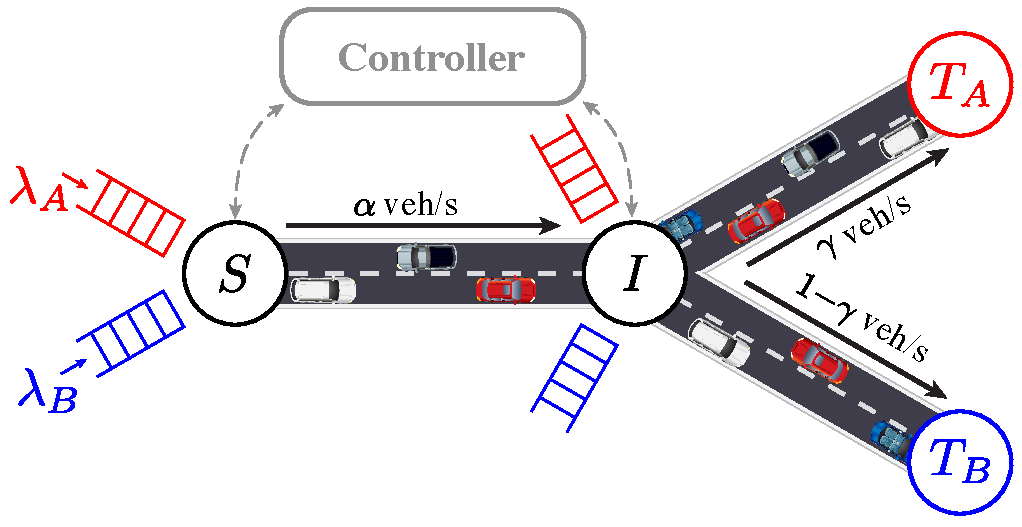
\includegraphics[width=\textwidth]{figures/simpleScenario.pdf}
        % }
        \caption{Two data transfers $A$ and $B$ originating from offloading spot $S$ share the road connecting offloading spot $I$. They then follow their own route toward their final destinations $T_A$ and $T_B$, respectively.}
        \label{fig:simple-scenario}
    \end{subfigure}%
    \quad %add desired spacing between images, e. g. ~, \quad, \qquad etc.
      %(or a blank line to force the subfigure onto a new line)
    \begin{subfigure}[t]{0.51\columnwidth}
        \centering
        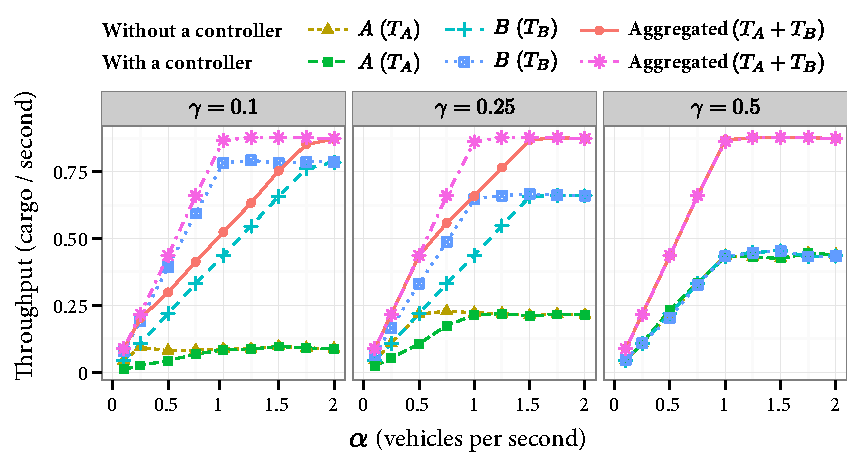
\includegraphics[width=\textwidth]{results/simpleScenario-throughput_v2_gamma_all.pdf}
        \caption{Maximum throughput (in number of data cargo received per second), for the two strategies with and without controller as a function of parameters $(\alpha,\,\gamma)$.}
        % (deduced from the AADT values)
        \label{fig:simple-scenario-throughput}
    \end{subfigure}
    \caption{Road network consisting in four offloading spots to show the benefits of having a controller.}
\end{figure}

We consider two scheduling strategies, without a controller and with a controller, to select the data transfer and to determine the amount of data to load on the vehicles stopping at each offloading spot. The first scheduling strategy (without a controller) selects the data cargo available at the offloading spots in a round-robin fashion. The data cargo of the transfers is selected in equal proportions and in circular order, without any priority given to the transfers. In the second strategy (with a controller), the decision to load a cargo on a vehicle is based on a pre-defined configuration of the offloading spots. The controller determines this configuration using the traffic volumes of road network under consideration. In the example of Figure~\ref{fig:simple-scenario}, if we assume the road traffic volume $I\rightarrow T_A$ to be three times greater than $I\rightarrow T_B$, the second strategy (with a controller) will load data three times more often onto vehicles heading to $T_A$. This is not the case of the strategy without a controller: this strategy will load the same amounts of data on stopping vehicles regardless of whether they head to $T_A$ or $T_B$.

We use \acrshort{sumo} (\acrlong{sumo}) to evaluate the three scheduling policies~\cite{behrisch2011sumo}. We simulate microscopic traffic in volumes of $\alpha$ vehicles per second from $S$ to $I$, $\gamma$ from $I$ to $T_A$, and $1 - \gamma$ from $I$ to $T_B$. We assume that both transfers $A$ and $B$ have infinite backlog of data at offloading spot $S$ (\ie $\lambda_A = \lambda_B = \infty$). Figure~\ref{fig:simple-scenario-throughput} shows the throughput of the system measured in the number of data cargo delivered to the destinations per second. In the scenario, the scheduling is relevant at $S$, as the road segments connecting the next-hop offloading spot $I$ to $T_A$ and $T_B$ exhibit different road traffic volumes. We consider an infinite backlog traffic generated at $S$ such that all vehicles leaving offloading spot $I$ are loaded with a cargo.

We can see that, for the first strategy without a controller, the transfer headed to $T_A$ needs a longer ramp-up period to reach its nominal throughput. Without any knowledge on the downstream traffic volumes, $S$ cannot load the optimal amounts of data to the next offloading spot $I$ to fully utilize the network resources. As a result, $I$ does not have enough data locally available to feed the higher flow of vehicles traveling towards $T_B$ compared to destination $T_A$. The resources available on the road segment $(I,\,B)$ remain underused when not enough data belonging to transfer $B$ are transported in an adequate amount to offloading spot $I$, \eg for $\alpha < 2$. On the contrary, the second strategy with controller allows $S$ to load data on vehicles traveling to $I$ in adequate amounts for both transfers. In turn, $I$ has enough data to efficiently utilize vehicles traveling on towards $T_A$ as well as $T_B$. The controller leverages the knowledge of traffic volumes on the downstream road segments to maximize the use of road resources at offloading spot $S$. This second strategy can achieve a better total throughput performance for all competing transfers at $I$. 

With this simple example, we showed the benefits of a centralized architecture that pre-configures the offloading spots to make the decisions to load data on vehicles. This architecture achieves better throughput compared to a distributed architecture decisions made locally at the offloading spots to load data on vehicles. In the following, we introduce a centralized architecture that controls a large-scale offloading infrastructure.

\clearpage
\section{Centralized controlled offloading architecture}
\label{sec:offloading-system-operations}

We exploit the logical centralization provided by \acrfull{sdn}\index{Software-Defined Networking (SDN)} to enable efficient control and management of the road network resources to offload bulk delay-tolerant traffic from a conventional data network. Following \acrshort{sdn}'s original design, our architecture consists of two components, as depicted in Figure~\ref{fig:architecture}: a central controller\index{controller} and the offloading spots acting as forwarding engines. We describe the function of each component in the remainder of this section. 

\begin{figure}[h]
	\centering
	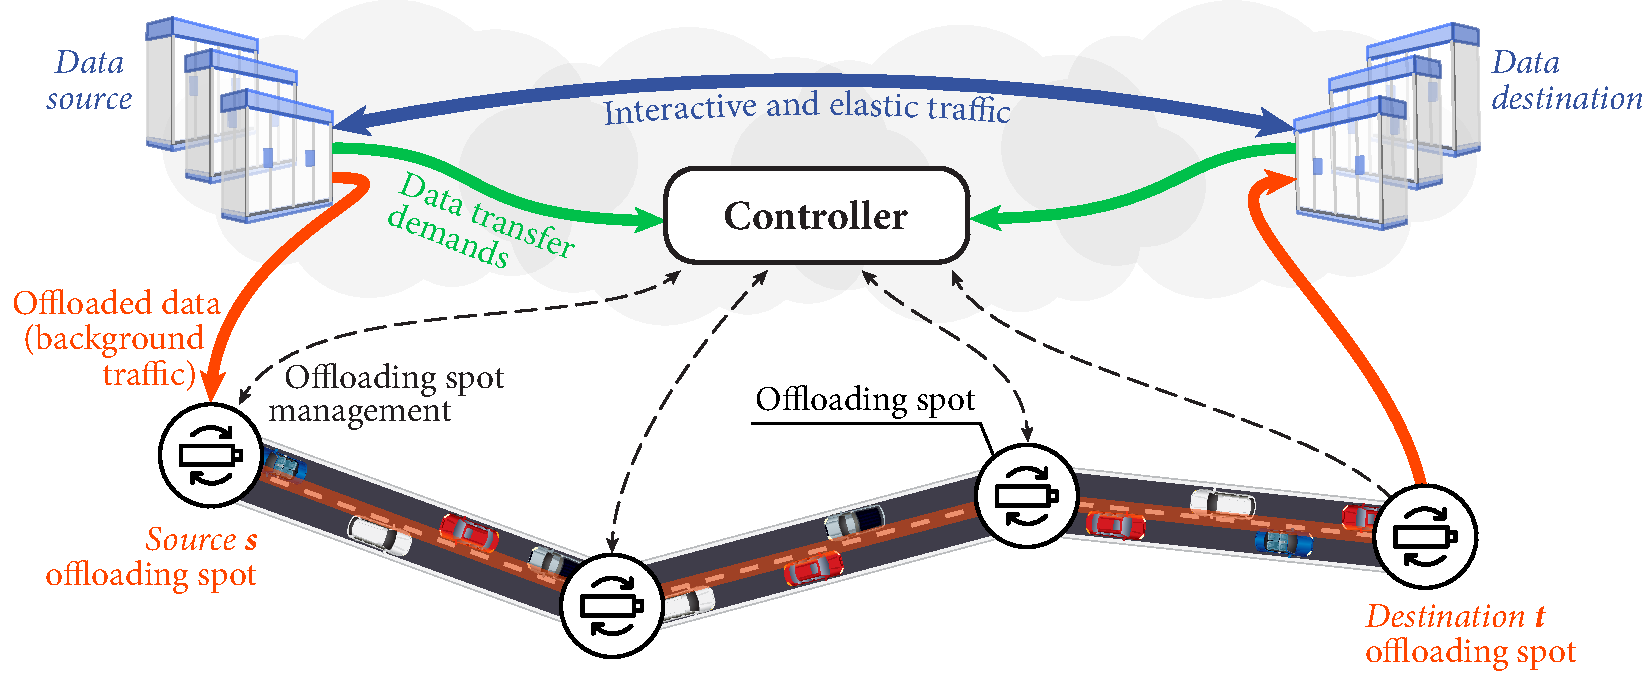
\includegraphics[width=0.85\columnwidth]{figures/architecture2.pdf}
	\caption{Centralized architecture to control the infrastructure in charge of offloading data.}
% 	In this scenario, the controller receives demands to offload bulk transfers of delay-tolerant data between two data centers. The controller configures the road network data plane by installing forwarding states at the offloading spots. The controller allocates the flows of vehicles on the roads connecting the offloading spots to carry the data towards its destination.}
	\label{fig:architecture}
\end{figure}




\subsection{Controller}

The controller\index{controller|bb} leverages the offloading overlay\index{offloading overlay} we presented in the previous chapter~\ref{sec:offloading-overlay}. As a result, the controller has a holistic view of the road network including its topology and dynamics, such as the traffic volumes for each road segment. Such knowledge may be derived from traffic forecasting services such as Navteq/Here\footnote{\url{https://www.here.com/business/traffic}},     
TomTom\footnote{\url{http://automotive.tomtom.com/en/connected-services/tomtom-traffic}}, or 
Airsage.\footnote{\url{http://www.airsage.com/Products/Traffic-Insights/}}. The controller keeps track of the status of the offloading spots via a long range control channel (\eg SigFox\footnote{\url{http://www.sigfox.com/}} or LoRa\footnote{\url{https://www.lora-alliance.org/}})~\cite{anteur2015ultra}. The information about the offloading spots includes the metadata of the data in transshipment and the statistics about the stopping vehicles, including the historical locations' made available via the navigation system of the vehicles. By collecting the information about the offloading spots, the controller has an up-to-date view of the offloading system. Recall that, in Section~\ref{sec:discuss}, we presented probabilistic tools to infer the remaining route of a vehicle knowing its navigation history, and the realization of the drayage system.

The controller receives demands\index{offloading demand} to offload data from transfers on the road network. Each demand specifies the delay and bandwidth requirements for the corresponding data transfer, as well as the origin and destination of the transfer. When receiving an offloading demand, the controller selects the road network paths by solving the vehicle flow allocation problem\index{vehicle flow allocation problem}. A road network path consists of a sequence of offloading spots followed by the data carried by vehicles between the offloading spots. In Section~\ref{sec:max-min-fairness-allocation-model}, we formulate the vehicle flow allocation problem as a \acrfull{lp} model that maximizes the throughput allocated in a fair manner to the flows of vehicles traveling between the consecutive offloading spots along the road network paths.

Figure~\ref{fig:controller-flowchart} shows the interactions between the functions of the controller with those of the offloading spots. The allocation procedure involves a reduction of the road network with the offloading overlay we detail in the next section. 

\begin{figure}[t]
	\centering
		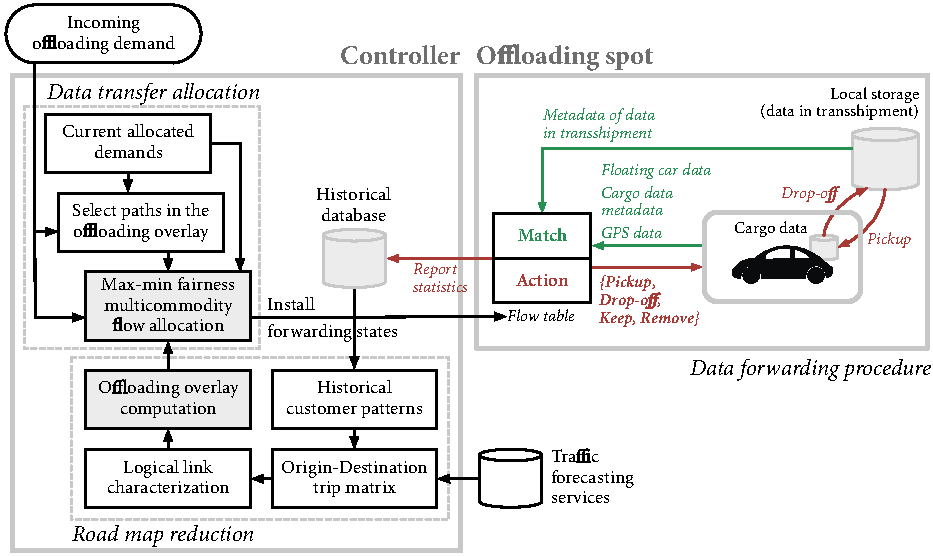
\includegraphics[width=\columnwidth]{figures/controller-flowchart-offloading-spot.pdf}
	\caption{Interactions between the functions of the controller and those of the offloading spots.}
	\label{fig:controller-flowchart}
\end{figure}


\subsection{Data forwarding at the offloading spots}
\label{sec:data-forwarding-offloading-spot}

We represent the interactions between the actions of the controller and the offloading spots in Figure~\ref{fig:controller-flowchart}. The controller installs forwarding states to control the local decisions made at the offloading spots to either drop off or pick up the data cargo. This decision results from the matching of the direction of the stopping vehicles against the destination of the available data. The local decisions account for the allocation of the road network resources shared among concurrent offloaded data transfers.

\clearpage

\begin{wrapfigure}[24]{o}[0.7\marginparwidth]{7.6cm}
    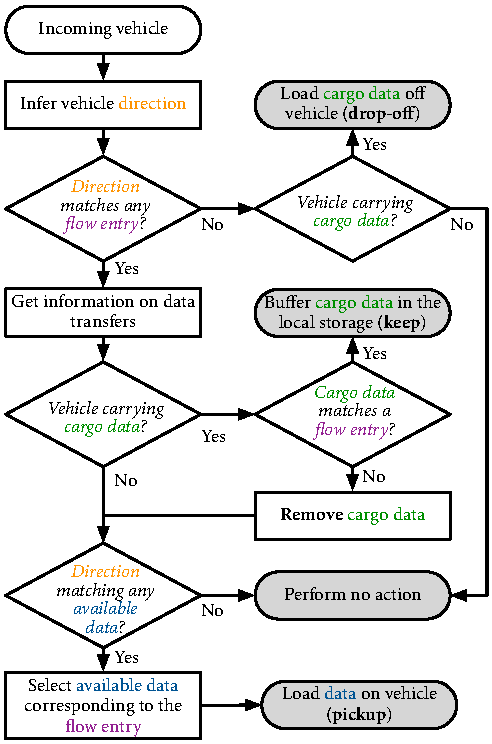
\includegraphics[width=7.5cm]{figures/forwarding.pdf}
    \caption{Forwarding process at an offloading spot.}
    \label{fig:forwarding-process}
\end{wrapfigure}
\paragraph{Flow tables.} 
The forwarding behavior of an offloading spot is determined by its \textit{flow table}\index{flow table|bb} represented in Figure~\ref{fig:controller-flowchart}. It consists of a list of entries, each installed for an individual offloading demands. The controller adds a new entry in the flow table of all the offloading spots on the road network path resulting from the allocation of a data transfer.
A flow entry contains the next-hop offloading spot to forward the data cargo along the allocated road path toward its destination.
% A flow entry forwards the data cargo to the next-hop offloading along the computed road path toward its destination.
% A flow table entry contains the next-hop offloading spot to which the data must be forwarded to reach the destination of the data transfer corresponding to this entry. 
The destination of the stopping vehicles is matched against the next-hop offloading spot of the flow entries. If there is a match, the offloading spot performs an action described by the forwarding process.
% on the cargo carried by the vehicle associated with the entry, including loading data on or off the vehicles.

\paragraph{Forwarding process.} 
The forwarding process is represented by the flowchart depicted in Figure~\ref{fig:forwarding-process}. Upon the arrival of a vehicle, an offloading spot checks if the direction of the vehicle matches one entry of its flow table. If none of the entries match, the vehicle unloads, if any, its data cargo onto the offloading spot storage for future pick-ups and continues its route without performing any further actions. If multiple entries match the direction of a vehicle, the offloading spot selects one entry based on the scheduling strategies presented in Section~\ref{sec:scheduling}. If the vehicle already carries data, the offloading spot checks if this data belongs to the data transfer represented by the matching entry. If this is the case, the vehicle keeps its cargo and continues its journey. Otherwise, the vehicle unloads its cargo at the offloading spots and becomes empty. For an empty vehicle, the oldest cargo associated with the selected entry is transferred to the vehicle.


\section{Max-min fair vehicle flow allocation model}
\label{sec:max-min-fairness-allocation-model}

In this section, we introduce the max-min fair allocation model\index{vehicle flow allocation problem!max-min fair allocation model|bb} solved by the controller in response to offloading demands. This model maximizes the throughput of the data flows allocated in a fair manner to the flows of vehicles traveling between the offloading spots. This model also integrates redundancy and retransmission mechanisms to completely recover from the effects of the logical link leakage. We then present the scheduling policies used by an offloading spot to serve concurrent data transfers. 

We consider the same assumptions regarding the offloading demands\index{offloading demand} as Section~\ref{sec:offloading-demands-feasibility} of the previous chapter. The demand is characterized by the amount of data $\beta_{st}$ and the deadline $\tau_{st}$ before which the transfer should be completed. However, here, we do not characterize the offloading demands with the leakage tolerance, since we target reliable transfers that do not tolerate any data losses. For simplicity, we model the rate of the demands at $s$ by a Poisson distribution $\lambda_{st}$ and its mean value is the average throughput $\beta_{st}/\tau_{st}$.

To improve the readability, we list the notations we use in the rest of this chapter in Table~\ref{tab:main-variables-haulage}. 

\begin{table}[ht]
    \caption{Table of notations for the max-min fair allocation model.}
    \renewcommand{\arraystretch}{1.1}
    \centering
    {\footnotesize
    \begin{tabular}{c|l}
        \textbf{Variable} & \textbf{Meaning}\tabularnewline
        \hline 
        $d_{st}$ & Offloading demand between source $s$ and destination $t$\tabularnewline
        $\tau_{st}$ & Deadline to transfer the data of offloading demand $d_{st}$\tabularnewline
        $\beta_{st}$ & Amount of data to transfer for offloading demand $d_{st}$\tabularnewline
        $\lambda_{st}$ & Poisson arrival rate at the source for offloading demand $d_{st}$\tabularnewline
        $\mathcal{P}_{st}$ & Set of simple paths between $s$ and $t$ on the offloading overlay\tabularnewline
        $\mathcal{S}$ & Storage capacity of the vehicles (cargo size)\tabularnewline
        $\mathcal{M}$ & Market penetration ratio\tabularnewline
        $c\left(i,\, j\right)$ & Capacity of logical link $\left(i,\, j\right)$\tabularnewline
        $t\left(i,\, j\right)$ & Travel time on logical link $\left(i,\, j\right)$\tabularnewline
        $l\left(i,\, j\right)$ & Leakage of logical link $\left(i,\, j\right)$\tabularnewline
        $l^{\textrm{\textbf{red}}}_{st}\left(i,\, j\right)$ & Leakage of logical link $\left(i,\, j\right)$ with redundancy for offloading demand $d_{st}$\tabularnewline
        $o^{\textrm{\textbf{red}}}_{st}$ & Weight of the \textbf{red}undancy mechanism on the data flow for offloading demand $d_{st}$\tabularnewline
        $R^{\{\textrm{hbh,e2e}\}}_{st}(i,\,j)$ & Average number of transmissions (either end-to-end (\textbf{e2e}) or hop-by-hop (\textbf{hbh}) \\
         & of a data cargo on logical link $(i,\,j)$ for offloading demand $d_{st}$\tabularnewline
        $\delta_{i}$ & Waiting time at offloading spot $i$ (to charge the EV's battery and load data)\tabularnewline
        $f\left(p\right)$ & Data flow on logical path $p$\tabularnewline
        $t\left(p\right)$ & Travel time of logical path $p$\tabularnewline
        $O_{st}(i,\,j)$ & Overhead of the offloading demand $d_{st}$ on the flow at logical link $(i,\,j)$\tabularnewline
        $R_{st}(i,\,j)$ & Number of transissions of a cargo belonging to demand $d_{st}$ on logical link $(i,\,j)$, \\
         & regardless of the retransmission mechanism\tabularnewline
    \end{tabular}}
    \label{tab:main-variables-haulage}
\end{table}

\subsection{Reliability overhead}
\label{sec:reliability}

In this section, we express the overhead in the throughput resulting from the two reliability mechanisms we consider. Firstly, we express the overhead for the redundancy mechanism in the case of RAID~6. Secondly, we express the overhead for the retransmission mechanism in the case of \acrfull{srarq}.

\subsubsection{\acrshort{raid} redundancy} 

Without loss of generality, we use \acrshort{raid}~6\index{reliability!RAID~6 redundancy} to partially recover from losses resulting from a vehicle failing to deliver its data cargo to the next offloading spot. \acrshort{raid}~6 divides the $\beta^{st}$ data of an offloading demand $d_{st}$ into $N$ arrays of $n\geq 4$ cargo. An array consists of two redundant cargo for $n-2$ cargo payloads. Therefore, a data transfer of $N$ RAID~6 arrays requires $nN$ vehicles, including $2N$ vehicles carrying redundant cargo to recover the losses in the $N(n-2)$ other vehicles.

\acrshort{raid} redundancy increases the amount of data sent by a factor $o_{st}^{\text{red}}$. For a data transfer involving exactly $n$ data cargo arranged in $N$ arrays, we express $o_{st}^{\text{red}}$ as follows:

\begin{equation}
	o_{st}^{\text{red}} = \frac{n}{n-2}\cdot
    \label{eq:redundancy}
\end{equation}

The data carried by $n$ vehicles whose storage devices are arranged in \acrshort{raid}~6 and travelling the logical link $(i,\,j)$ experiences a reduced data leakage denoted $l^{\text{red}}_{st}(i,\,j)$. We express $l^{\text{red}}_{st}(i,\,j)$ in terms of $l(i,\,j)$ (\ie the data leakage $(i,\,j)$ without data redundancy protection) as follows:

\begin{equation}
	l^{\text{red}}_{st}(i,\,j) = 1 - \sum_{k=0}^{2} \binom{n}{k} l(i,\,j)^{k}\big(1-l(i,\,j)\big)^{n-k}.
\end{equation}

\noindent Note that this expression assumes a data linkage equivalent to the failure likelihood of a storage device, which is consistent as both are independent and identically distributed. 

We explain how we determine $n$ (the number of storage devices per array) at the end of this section, as it depends on the total amount of transmitted data (including redundant data and the additional copies introduced by the retransmissions for recovering losses that \acrshort{raid} cannot repair). 

% We propose two retransmission strategies, as depicted in Figure~\ref{fig:global-architecture}: hop-by-hop (hbh) retransmissions and end-to-end (e2e) retransmissions. With the hop-by-hop strategy\index{Reliability!SR-ARQ Retransmission}, each offloading spot buffers data for later recovery in case a vehicle fails to deliver its cargo to the next-hop offloading spot. The controller receives acknowledgments over a feedback channel from the next-hop offloading spot (indicated by dashed arrows 2b-4b in Figure~\ref{fig:global-architecture}) and notifies through the same channel the previous offloading spot when to retransmit the missing data. With the end-to-end strategy (indicated by dashed arrows 1a and 4b in Figure~\ref{fig:global-architecture}), the only offloading spots in charge of recovering a loss are the edge offloading spots where the data is first transloaded from the computer network and stored until successfully transmitted. After a predefined number of attempts, a loss is repaired via the original data network (from where data was first transloaded) to make sure the deadline specified in the offloading demand can be met. Communication between the controller and the offloading spots incurs low bandwidth overhead and may be handled via a legacy data network (\eg the Internet). 

% \begin{wrapfigure}[27]{o}[0.7\marginparwidth]{7.6cm}
%     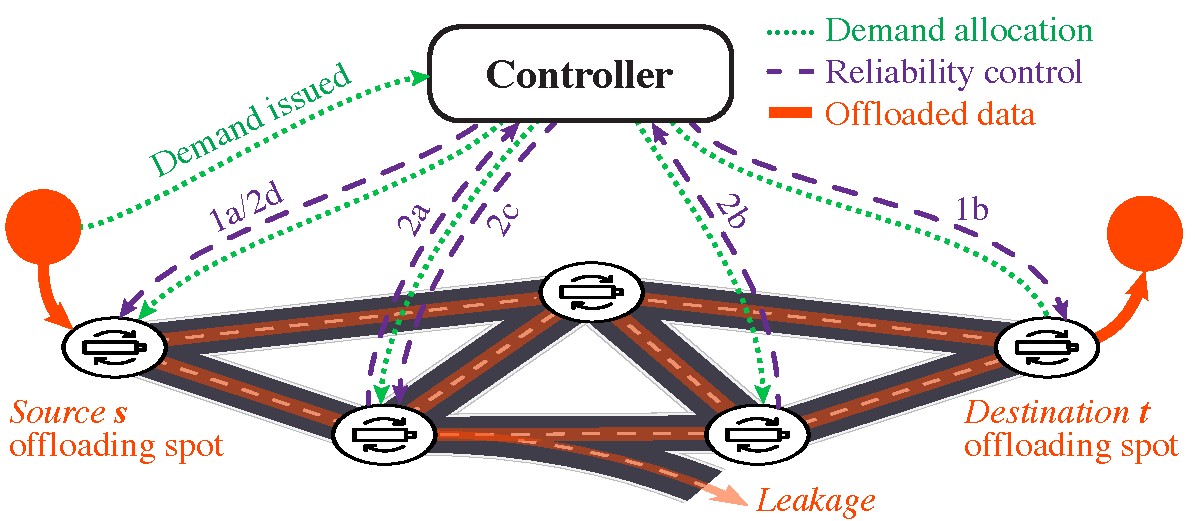
\includegraphics[width=7.5cm]{figures/architecture3.pdf}
%     \caption{A legacy data network (\eg access wired or wireless network) is used to transmit control messages between the offloading spots and the controller. The control channels allow the controller to access and change the forwarding behavior of the offloading spots (dotted arrows). Controller-to-offloading spot communication is also used for the end-to-end retransmission strategy (dashed arrows 1a, 4b) and the hop-by-hop retransmission strategy (dashed arrows 1a-3a and 2b-4b).}
%     \label{fig:architecture-retransmissions}
% \end{wrapfigure}

\begin{figure*}[!t]
    \centering
    \begin{subfigure}[b]{0.45\textwidth}
        \centering
        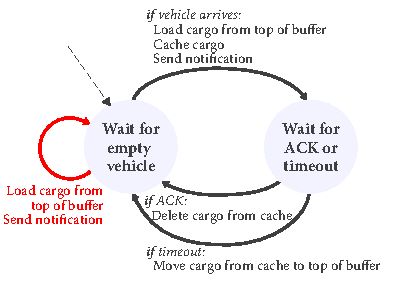
\includegraphics[height=5cm]{figures/retransmissions-sender.pdf}
        \caption{Sender-side (offloading spot $i$).}
        \label{fig:retransmissions-sender}
    \end{subfigure}%
    \qquad
    \begin{subfigure}[b]{0.45\textwidth}
        \centering
        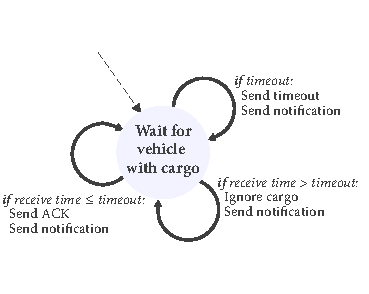
\includegraphics[height=5cm]{figures/retransmissions-receiver.pdf}
        \caption{Receiver-side (offloading spot $j$).}
        \label{fig:retransmissions-receiver}
    \end{subfigure}%
    \caption{\acrshort{srarq} retransmissions. The red transitions is exclusively for the intermediate offloading spots in case of end-to-end retransmissions. The other transitions is for the source offloading spot in case of end-to-end retransmission and the source and the intermediate offloading spots in case of hop-by-hop retransmission.}
    \label{fig:retransmissions}
\end{figure*}

\subsubsection{\acrshort{srarq} retransmissions}

In addition to data redundancy, we use \acrfull{srarq}\index{reliability!SR-ARQ retransmissions} to fully recover the losses that \acrshort{raid} cannot recover~\cite{costello2004error}. We propose two retransmission strategies: hop-by-hop (hbh) retransmissions and end-to-end (e2e) retransmissions. In Figure~\ref{fig:retransmissions}, we represent the sender-side in Figure~\ref{fig:retransmissions-sender} and the receiver-side in Figure~\ref{fig:retransmissions-receiver}. The red transition in the sender-side refers to the behavior of the intermediate offloading spots in case of end-to-end retransmissions, while the other transitions refer to the behavior of the source offloading spot in case of end-to-end retransmission and all the offloading spots in case of hop-by-hop retransmissions. The controller enforces the retransmissions at the offloading spots using a low-bandwidth control channel\index{control channel}. Both retransmissions strategies rely on timeout expiration\index{reliability!SR-ARQ retransmissions!timeout} at the receiver-side to trigger a retransmission. The timeout corresponds to the travel time $t(i,j)+\varepsilon$ ($\varepsilon$ constant) between two offloading spots $i$ and $j$ and depends on the current road traffic. Note that, the controller can also leverage traffic forecasting services to re-evaluate the travel time using exponential weighted moving average techniques.

With the hop-by-hop strategy\index{reliability!SR-ARQ retransmissions!hop-by-hop}, the controller is informed of loaded vehicles leaving offloading spot $i$. A copy of the cargo is cached by $i$ until successfully transmitted to $j$, the next-hop offloading spot. If no acknowledgment is received from $j$ before the timeout expires, the controller notifies $i$ to retransmit the missing cargo.  The hop-by-hop strategy introduces an overhead corresponding to the average number of transmissions $R^{\textrm{hbh}}_{st}(i,\,j)$ needed to successfully deliver a cargo on logical link $(i,\,j)$. We express $R^{\textrm{hbh}}_{st}(i,\,j)$ as follows:
\begin{equation}
    R_{st}^{\textrm{hbh}}(i,\,j) =  \frac{1}{1-l_{st}^{\text{red}}(i,\,j)}\cdot
\end{equation}

With the end-to-end strategy\index{reliability!SR-ARQ retransmissions!end-to-end}, the only offloading spot in charge of recovering a data loss is the first one located at the source-side of the data transfer. Once the last offloading spot on the destination-side receives the data, it notifies the controller of the successful delivery. In turn, the controller notifies the first offloading spot on the source-side to delete the cached copy of the cargo. If the intermediate offloading spots do not receive the expected cargo before the timeout expires, they notify the controller, which in turn asks the source to send another copy of the cargo. The overhead of the end-to-end strategy corresponds to $R^{\textrm{e2e}}_{st}(i,\,j)$, the average number of transmissions of a cargo on logical link $(i,\,j)$ before successfully delivering it from $s$ to $t$. We express $R^{\textrm{e2e}}_{st}(i,\,j)$ as follows:
\begin{equation}
    R^{\textrm{e2e}}_{st}(i,\,j) = \frac{(-1)^{n-(i-1)}}{\prod_{j=i}^{n-1}\big(l_{st}^{\text{red}}(j_{i},\,j_{i+1})-1\big)}\cdot
\end{equation}

We denote $O_{st}(i,\,j)$ as the total overhead introduced by \acrshort{raid}~6 and \acrshort{srarq} on logical link $(i,\,j)$ to recover from vehicles failing to deliver the data sent with offloading demand $d_{st}$. We express $O_{st}(i,\,j)$ in terms of the overheads introduced by both the redundancy and retransmission mechanisms as follows:
\begin{equation}
    O_{st}(i,\,j) = \begin{dcases}
    o_{st}^{\text{red}} \times R_{st}^{\textrm{hbh}}(i,j) & \text{\!\!\small (hop-by-hop)}\\
    o_{st}^{\text{red}} \times R_{st}^{\textrm{e2e}}(i,j) & \text{\!\!\small (end-to-end)}
    \end{dcases}
\end{equation}
\noindent where $o_{st}^{\text{red}}$ is given by Equation~\ref{eq:redundancy}.

In the following, we will use $o^{\text{ret}}_{st}(i,\,j)$ to represent the overhead of the retransmission mechanism regardless of whether the mechanism is hop-by-hop or end-to-end. Similarly, we use $R_{st}(i,j)$ to represent the number of transmissions on logical link $(i,j)$ for cargo belonging to demand $d_{st}$, regardless of the retransmission mechanism.

\subsubsection{Determination of the array size $n$} 

\Acrshort{raid}~6 redundancy distributes the data across arrays of $n$ data cargo. The total number of data cargo $n$ is defined so that to minimize the data overhead $O_{st}$ needed to ensure reliable transfer in response to offloading demand $d_{st}$: 
\[
    \min O_{st}=\begin{dcases}
    \min_{n} \left\{ o_{st}^{\text{red}} \times \max_{(i,\,j)\in p}\{R_{st}^{\textrm{hbh}}(i,j)\} \right\} & \text{\!\!\small (hop-by-hop)}\\
    \min_{n} \left\{ o_{st}^{\text{red}} \times  \max_{(i,\,j)\in p}\{R_{st}^{\textrm{e2e}}(i,j)\} \right\} & \text{\!\!\small (end-to-end)}
    \end{dcases}
\]


\subsection{Max-min vehicle flow allocation model}
\label{sec:max-min-allocation-model}

The controller receives the demands to offload data transfers characterized by their performance requirements. The task of the controller consists in selecting the flows of vehicles according to the following constraints: (\textit{i}) the number of vehicles is sufficient to meet the transfer requirements and (\textit{ii}) the allocation of the combined storage of the vehicles is efficient and fair among the competing transfers. To this end, the controller starts by computing the logical paths in the offloading overlay for each of the transfer to offload. The controller then allocates flows of data on these paths while satisfying both constraints and finally configures then the offloading spots along the selected logical paths with a non-zero allocation.

In the following, $\mathcal{P}_{st}$ denotes the set of candidate logical paths between $s$ and $t$. Each logical path $p\in\mathcal{P}_{st}$ consists of a sequence of logical links connecting pairs of offloading spots in the offloading overlay. We express the path travel time\index{logical path!travel time} $t(p)$ experienced by a data transfer allocated to flows of vehicles traveling on logical path $p$ belonging to the set of logical paths $\mathcal{P}_{st}$ for offloading demand $d_{st}$. The path travel time is the sum of two components: travel time component and waiting component. The travel time component is the sum of the travel time of the logical link of $p$. The waiting component is the sum of the waiting times at each offloading spot connecting these logical links. We express $t(p)$ as a function of $R_{st}(i,j)$, the average number of transmissions of a cargo to successfully deliver it from $i$ to $j$ for demand $d_{st}$:
\begin{equation}
    \label{eq:impl-logical-path-travel-time}
	t\left(p\right) = \sum_{\substack{p\in \mathcal{P}_{st}\\(i,\, j)\in p}} R_{st}(i,\,j)\left[\delta_{i} + t(i,\,j)\right],
\end{equation}
\noindent where $\delta_i$ is the waiting time at offloading spot $i$.


\subsubsection{Linear programming formulation} 

We formulate the vehicle flow allocation procedure as a \acrfull{lp} model that determines the logical paths matching the performance requirements of the offloading demands. The \acrshort{lp} shown in Algorithm~\ref{fig:allocation} consists in allocating $f(p)$ data to the flows of vehicles traveling the logical paths of $\mathcal{P}_{st}$. We first present the inputs and then the allocation strategy for the offloading demands. The strategy relies on the multi-commodity flow allocation problem we formulate as a linear programming model. 

% \removelatexerror% Nullify \@latex@error
\begin{algorithm*}[H]
	\KwIn{Offloading demands $\mathcal{D} = \{d_{st}\}$, characterized by $\beta_{st}$ and $\tau_{st}$}
    \myinput{Set $\{\mathcal{P}_{st}\}_{st}$ of the logical paths between $s$ and $t$ for each demand in $\mathcal{D}$}
    \myinput{Average travel time $t(p)$ on logical path $p$}
    \myinput{Capacity $c(i,\,j)$ of logical link $(i,\,j)$}
    
    \KwOut{Resulting allocation $A=\{f(p)\}$ of flows to logical paths $p$}
    
    \BlankLine
    \Proc{\Alloc}{
        $L \gets \{\textrm{Logical links } (i,\,j)\}$\;
        $\{f(p)\} \gets \textsf{Max-Min Fairness(}\mathcal{D},\,L\textsf{)}$\;
        \Return{$\{f(p) : p\in \mathcal{P}_{st},\, (s,\,t)\in \mathcal{D}\}$}
    }
    
    \BlankLine
    \Func{\MaxMin{$\mathcal{D},\,L$}}{
    	\textit{Initialization:} $U\gets \mathcal{D};\;i\gets 0;\;A\gets\emptyset$\;
    	\While{$U\neq \emptyset$}{
    		\textit{Maximize the $i$-th smallest allocation:}\;
    		\Indp 
    	      $\phi_{i} \gets \MCF{$\mathcal{D},\,C,\,U,\,i,\,A$}$\;
    		\Indm
    		\textit{Perform non-blocking test:}\;
    		\Indp 
			  $A_{i} \gets \NBT{$U,\,A,\,\phi_{i}$}$\;
    		\Indm 
    		Fix the allocation of each demand in $A_{i}$ to $\phi_{i}$\;
    		$U\gets U\backslash A_{i}$\;
    		$i\gets i+1$\;
    	}
    	\Return{$\{f(p) : p\in A\}$}\;
    }
    
    \BlankLine
    \Func{\MCF{$D,\,C,\,U,\,i,\,A$}}{
        $\begin{array}{cc}
		\textrm{Maximize} & \phi_{i}\end{array}$\\
		$\begin{array}{ll}
		\textrm{Subject to:} & \\
		\sum_{p}f(p)\big(\tau_{st} - t(p)\big) \geq \beta_{st} & \forall(s,\,t)\in \mathcal{D}\\
		\phi_{i} - \sum_{p} f(p)\big(\tau_{st} - t(p)\big) \leq 0 & \forall(s,\,t)\in U\\
		\phi_{k} - \sum_{p} f(p)\big(\tau_{st} - t(p)\big) = 0 & \forall(s,\,t)\in A_{k}, \phi_{k} \textrm{ constant},\\
	    & k = 0,\,\dotsc,\,i-1\\
		\sum_{s,\,t} o^{\text{red}}_{st} \sum_{p} \big[ o^{\text{ret}}_{st}(i,\,j) f(p) \big] \leq c(i,\,j) & \forall(i,\, j)\in L,\\
		& p\textrm{ s.t. }(i,\,j)\in p\\
		\end{array}$\;
		\Return{$\{\phi_{i}\}\cup \{f(p) : p\in \mathcal{P}_{st},\, (s,\,t)\in \mathcal{D}\}$}\;
    }
    \caption{Computing the allocations with the max-min fair allocation model\index{vehicle flow allocation problem!max-min fair allocation model}.}
    \label{fig:allocation}

\end{algorithm*}

\paragraph{Inputs.} 
The model takes as input the set $\mathcal{D}$ of all demands to offload a data transfer on the road network. This set includes the previous demands already allocated in addition to the new demands.\footnote{We have to re-allocate the previous demands to guarantee fair allocation of these demands and the new ones.} The allocation procedure also takes as input $\mathcal{P}_{st}$, the set of candidate logical paths between each pair $s$ and $t$ for all demands in $\mathcal{D}$. To enumerate the logical paths in $\mathcal{P}_{st}$, we propose to use Yen's $k$-shortest paths algorithm~\cite{yen1971finding} or a breadth-first search algorithm~\cite{lee1961algorithm}. In our simulations, we reduce the search space by considering the logical paths sorted according to the travel time of a single cargo. The offloading overlay and the properties of each logical link (\ie capacity, travel time, and data leakage) are also inputs of the allocation procedure.

\paragraph{Model.} 
The controller allocates $f(p)$ flows to the logical paths listed in $\mathcal{P}_{st}$ according to the \textsf{Max-Min fairness}\index{max-min fairness model|bb} strategy. This strategy proceeds by successive iterations.  The first iteration allocates the minimum flows to satisfy the requirements of the demands (given by the first constraint in the \textsf{MCF} function). The next iterations successively allocate the remaining capacity of the network to the demands that can receive more flow. More specifically, iteration $i$ maximizes the minimal flow allocation noted $\phi_{i}$ and fixes the allocation for the demands that cannot be better served, \ie because of the capacity constraints of the paths or if the demand requirements are already satisfied. The next iterations process the remaining demands. To determine for which transfers the current allocation can be further increased in the following iterations, we use the non-blocking test algorithm presented shown in Algorithm~\ref{fig:NBT}. 


% \removelatexerror% Nullify \@latex@error
\begin{algorithm*}[h!]
	\KwIn{Set $U$ of demands allocated at step $i$}
	\myinput{Set $A$ of demands allocated at steps $k<i$}
	\myinput{Allocation $\phi_{i}$ of step $i$}
	\KwOut{Set $A_{i}$ of flows in $U$ that cannot be allocated more than $\phi_{i}$ in any solution}
    
    \BlankLine
    \Func{\NBT{$U,\,A,\,\phi_{i}$}}{
        \textit{Demands that have been satisfied are allocated:}\;
        \Indp 
            $D_{i} = \{(s,\,t) \textrm{ s.t. } \sum_{p}f(p)\big(\tau_{st} - t(p)\big) = \beta_{st} \}$\;
            $U \gets U \backslash D_{i}; \; A_{i} = D_{i}$ \;
        \Indm
        \textit{Demands allocated more than $\phi_{i}$ can be increased:}\;
        \Indp 
            $U_{i} \gets \{(s,\,t) \textrm{ s.t. } \sum_{p}f(p)\big(\tau_{st} - t(p)\big) > \phi_{i} \}$\;
        \Indm
        \textit{Test the allocation of the remaining demands:}\;
        \ForEach{demand $(s,\,t)\in U\backslash (A_{i}\cup U_{i})$}{
            $\begin{array}{@{}ll@{}}
            \textit{Solve the following linear program:} & \\
    		\textrm{Maximize} & \sum_{p\in\mathcal{P}_{st}} f(p)\\
    		\textrm{Subject to:} & \\
    		\sum_{p}f(p)\big(\tau_{st} - t(p)\big) \geq \beta_{st} & \forall(s,\,t)\in D\\
    		\phi_{k} - \sum_{p} f(p)\big(\tau_{st} - t(p)\big) = 0 & \forall(s,\,t)\in A_{k}, \phi_{k} \textrm{ constant}, \\
    	    & k = 0,\,\dotsc,\,i-1\\
    		\sum_{s,\,t} o^{\text{red}}_{st} \sum_{p} \big[ o^{\text{ret}}_{st}(i,\,j) f(p) \big] \leq c(i,\,j) & \forall(i,\, j)\in C,\\
    		& p\textrm{ s.t. }(i,\,j)\in p\\
    		\end{array}$\;
    		
            \lIf{$\sum_{p\in\mathcal{P}_{st}} f(p) \leq \phi_{i}$}{
                $A_{i} \gets A_{i}\cup \{(s,\,t)\}$\;
            }
            \lElse{$U_{i}\gets U_{i} \cup \{(s,\,t)\}$}\;
        }
        
        \Return{$A_{i}$}\;
    }
    
    \caption{Non-blocking test for the max-min fairness allocation model.}
    \label{fig:NBT}
\end{algorithm*}

The core of the max-min fairness algorithm is the \textsf{MCF} (\acrshort{mcf}) function shown in Figure~\ref{fig:allocation}. The \textsf{MCF} function computes the multi-commodity flow allocation\index{multi-commodity flow allocation} for the remaining demands. The first constraint matches the amount of data that can be offloaded within the deadline $\tau_{st}$ to the amount of data to transfer $\beta_{st}$. The following constraint ensures that the demands belonging to the sets $A_{k},\,k\in [0,\,i-1]$ are fixed to the allocation they received at previous step $k$. The objective of the \textsf{MCF} function is to maximize the minimum allocation $\phi_{i}$ such that all demands are satisfied. This objective is further guaranteed by the third constraint of the linear problem. Finally, the last constraint limits the total allocation of the paths crossing the logical links to the logical link capacity. Note that this constraint takes the overhead of the retransmission and the redundancy mechanisms into account. 

Once the allocation $\phi_i$ have been fixed by the \textsf{MCF} function for iteration $i$, the max-min fairness algorithm determines which demands can be further increased in their current allocation using the non-blocking test algorithm shown in Figure~\ref{fig:NBT}. The non-blocking test is derived from the algorithm proposed by Pi\'{o}ro \etal~\cite{pioro2003efficient}. This test compares the maximal throughput of the flows allocated by a multi-commodity flow allocation to the one resulting from the minimal flow allocation $\phi_{i}$. If the multi-commodity flow allocation improves the maximal amount of data allocated to a demand, the demand will be fixed in the next iterations of the max-min fairness algorithm. Otherwise, the demand cannot be better increased, and it is fixed to $\phi_{i}$. 

Note that the formulation of the multi-commodity flow remains valid for continuous flows (infinite backlog data traffic). In this case, we ignore the first constraint in the \textsf{MCF} function that satisfies the demand requirements.

The max-min fair allocation model presented in this section has a polynomial time-complexity because fractional flows are allowed in the linear programming models formulated in function \textsf{MCF} and the non-blocking algorithm~\cite{karakostas2008faster}. The time-complexity of both linear programming models grows in linear time with the number of demands and the number of paths in $\mathcal{P}_{st}$ for each demand $d_{st}$ of the set of demands to allocate. 

\subsection{Data scheduling} 
\label{sec:scheduling}

Recall from Section~\ref{sec:data-forwarding-offloading-spot} that offloading spots use flow tables to match the data locally available with the stopping vehicles and decide an action to take. Multiple entries in the flow table of an offloading spot $i$ may match the direction of a vehicle. Each entry corresponds to different data transfers or the same transfer spanning many paths in the road network. The offloading spot selects in which order the flow of vehicles should be allocated to the transfers according to the weighted fair queuing scheduling policy whose weights are configured by the controller, resulting from the allocation procedure output. We denote by $f(d_kp_l)$ the data flow on logical path $p_l$ allocated to the transfer resulting from offloading demand $d_k$. The controller assigns a weight $w(d_kp_l)$ to the transfers allocated to the logical paths in $P = \{d_kp_l | \forall d_k\in D,\, p_l\in \mathcal{P}^{d_k},\, (i,\,j) \in p_l\}$. $P$ is the set of logical paths passing by offloading spot $i$ and sharing the same next-hop offloading spot $j$. The controller computes $w(d_kp_l)$ by normalizing the rate of flow $f(d_kp_l)$ with the total rate of the flows traveling all paths in $P$:
\begin{equation}
    w(d_kp_l) = \frac{f(d_kp_l)}{\sum_{p\in P} f(p)}\cdot
\end{equation}

We use the weights in the scheduling algorithm to determine the priority of data transfers to assign the corresponding data cargo to a passing vehicle if multiple transfers traverse the same offloading spot. In our simulations, we considered a probabilistic weighted fair queuing scheduler, which uses the weights to pick a data transfer at random and assign the corresponding cargo to the stopping vehicle~\cite{shreedhar1996efficient}.


\section{Performance evaluation on the French road network}
\label{sec:throughput-max-model-eval}

In our evaluation, we use the same dataset\index{French road network} as the one we used in the previous chapter to conduct the evaluation of the throughput resulting from the cost-benefit maximization of offloading data (refer to Section~\ref{sec:res-revenue-max-model}).

We provide a characterization of the offloading overlay introduced in Section~\ref{sec:road-map-reduction-throughput} using more comprehensive road traffic modelling techniques compared to Section~\ref{sec:eval-offloading-overlay} to estimate the road traffic volumes between the offloading spots. Secondly, we evaluate the max-min fair allocation model we introduced in Section~\ref{sec:max-min-allocation-model} using the dataset of the French roads.

\subsection{Road map reduction} 
\label{sec:road-map-reduction-throughput}

\begin{wrapfigure}[13]{o}[0.7\marginparwidth]{8cm}
    \vspace{-15pt}
    \centering
    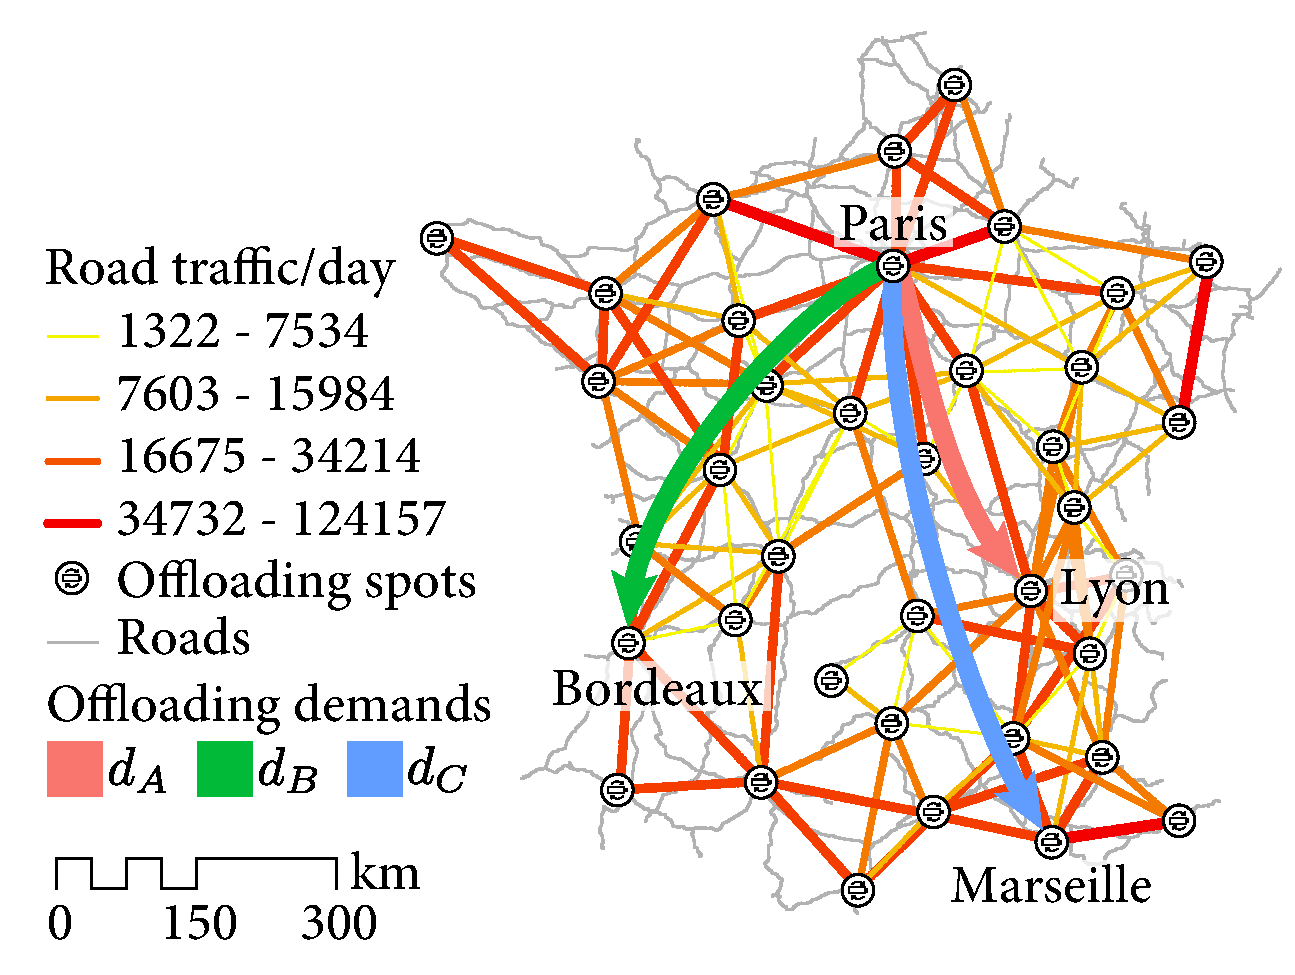
\includegraphics[width=7.5cm]{figures/France-overlay-haulage.pdf}
    \caption{Schematic representation of the demands $d_A$, $d_B$, and $d_C$.}
    \label{fig:france-demand-allocation-haulage}
\end{wrapfigure}
In the following, we characterize the logical links of the offloading overlay by expressing the road traffic volumes between adjacent offloading spots in terms of network quantities. These volumes are given by origin-destination matrices between the offloading spots. However, the datasets we use in our simulations only give the traffic counts in terms of \acrshort{aadt} (\ie the number of vehicles per unit of time for each road segment). We discuss the reasons why we use traffic counts in Section~\ref{sec:discuss-haulage}.

We use well-known traffic modelling techniques from transportation research to estimate the origin-destination matrix of the offloading spots from the traffic counts of the dataset\index{traffic modelling techniques}. We detail the traffic modelling techniques in the Appendix~\ref{cha:traffic-forecasting-techniques}. We proceed with the following three steps.

\begin{enumerate}

    \item \textit{Route determination.} The first step consists in selecting a subset of the alternative routes (to the shortest one) connecting each pair of adjacent offloading spots in the road network. The selection consists in choosing the $k$-shortest routes in terms of travel time. The routes are also selected such that they share a low degree of similarity in terms of stretches of road in common. We implement this selection process by using the algorithms proposed by Abraham \etal~\cite{abraham2013alternative}.

    \item \textit{Route assignment.} The second step consists in assigning weights to the selected routes using the C-logit route assignment model~\cite{cascetta1996modified}. The value of a weight is determined according to properties such as the travel time and the distance of the route. Those weights reflect the capacity of a route in attracting traffic, the higher the weight of a route the more traffic it will receive. The weights are then used in combination with the traffic counts to estimate the traffic volume of the routes selected in the first step between each pair of adjacent offloading spots. 
    
    \item \textit{Trip matrix estimation.} In the third step, we use the entropy maximization model proposed by Zuylen and Willumsen to compute the origin-destination trip matrix consisting in all pairs of offloading spots in the offloading overlay~\cite{van1980most}. This model determines the most likely distribution of the traffic across all the routes selected in Step~1 subjected to two constraints, namely the traffic counts of the routes' stretches of road and the C-logit weights. We feed this model with a dataset of the French roads we consider to infer the \acrshort{od} trip matrix between the adjacent offloading spots. 
    
\end{enumerate}

Finally, we determine the attributes of each logical link $(i,\,j)$ in the offloading overlay. These attributes are relevant to the allocation of the data transfers. The attributes are as follows:
\begin{itemize}

    \item \textit{Capacity $c(i,\,j)$.} The capacity of $(i,\,j)$ represents the combined storage of all vehicles travelling between $i$ and $j$. The capacity also reflects the market penetration ratio $\mathcal{M}$\index{market penetration ratio}, \ie the ratio of vehicles equipped with data storage devices.
    
    \item \textit{Travel time $t(i,\,j)$.} The travel time is computed as the travel time average for each route selected in the first step  between $i$ and $j$ and weighted by the route weights computed in the second step.
    
    \item \textit{Leakage $l(i,\,j)$.} The leakage represents the ratio of vehicles that fail to deliver the data they transport to the next offloading spot.
    
\end{itemize}

% We use the road traffic foresting techniques introduced in Section~\ref{sec:mapping-offloading-overlay} to estimate the road traffic on the logical links connecting pairs of offloading spots on the offloading overlay. We represent the resulting offloading overlay in Figure~\ref{fig:france-demand-allocation-haulage}. With this techniques, we have more realistic traffic flows between the offloading spots compared to the technique we used in Section~\ref{sec:res-revenue-max-model}.

% We connect neighboring charging stations via a set of disjoint alternative routes selected in the road map of France by running the algorithms proposed by Abraham \etal~\cite{abraham2013alternative} (refer to Section~\ref{sec:route-determination}). Selected routes share up to 80\% with the shortest route, while their length is at least 80\% of the shortest route. To estimate traffic volumes, we use the C-logit traffic assignment model~\cite{cascetta1996modified} (refer to Section~\ref{sec:route-assignment}). This model assigns a weight to the routes connecting the pairs of offloading spots less than 300~km away (\ie the driving range of an electric vehicle). We use the entropy maximization model\index{origin-destination trip matrix} proposed by Zuylen and Willumsen~\cite{van1980most} to infer the origin-destination traffic matrix consisting of all pairs of offloading spots (refer to Section~\ref{sec:trip-matrix-estimation}).


\subsection{Max-min fair allocation model on the roads of France} 

The objective of the simulation is to evaluate three metrics: (\textit{i}) maximum throughput of the resulting allocation to evaluate the capacity of the offloading infrastructure, (\textit{ii}) delay to transfer pre-defined amounts of data depending on the number of offloading spots involved in the data transfers and (\textit{iii}) fairness of the allocation of concurrent transfers when using logical paths with similar lengths.

We evaluate the performance of the transfers resulting from the allocation of three offloading demands using the max-min fair allocation model. The three demands are shown in Figure~\ref{fig:france-demand-allocation-haulage}: (\textit{i}) $d_A$ from Paris to Lyon with arrival rate $\lambda_A$, (\textit{ii}) $d_B$ from Paris to Bordeaux with arrival rate $\lambda_B$, and (\textit{iii}) $d_C$ from Paris to Marseille with arrival rate $\lambda_C$. Note that the road paths followed by the transfers resulting from demands $d_A$ and $d_C$ share the same logical links in the offloading network; as so $d_A$ and $d_C$ are competing over those links.  We use \acrshort{sumo} to run the simulations, which each lasts 300,000~seconds (3.5~days), including 43,200~seconds (12~hours) of \textit{warmup}, to give time for the first data cargo to reach their respective destination. In the rest of this section, we consider a conservative market penetration ratio $\mathcal{M}$ of 10\%\index{market penetration ratio}. Data leakage is assumed to be the same for all logical links in the offloading overlay. 

\subsubsection{Maximum throughput}

\begin{figure}[h!]
    \centering
    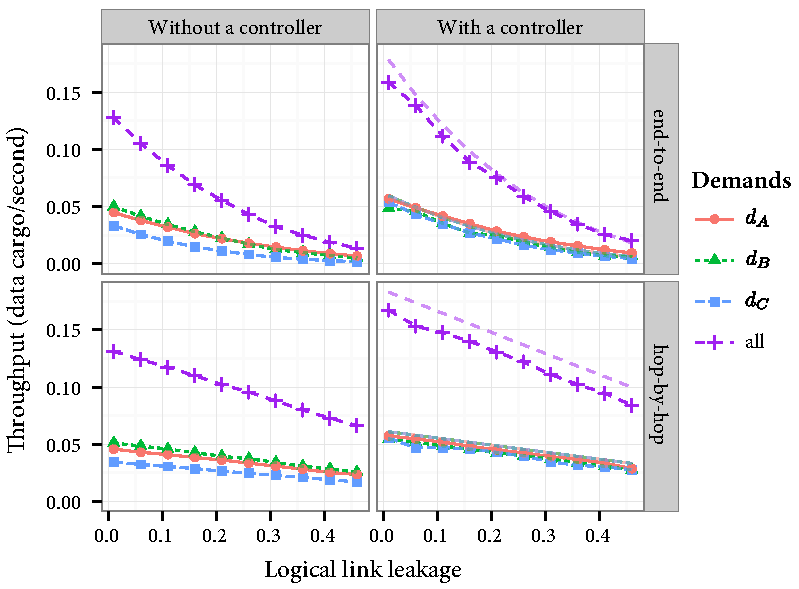
\includegraphics[width=0.65\textwidth]{results/plot-france-rate-throughput-m-10-wo-MCF.pdf}
    \caption{The maximum throughput achieved for offloading demands $d_A,\,d_B$ and $d_C$ (depicted in Figure~\ref{fig:france-demand-allocation-haulage}) as a function of the logical link data leakage (assumed to be the same on all the logical links).}
    \label{fig:french-net-throughput-leakage}
\end{figure}

We evaluate the maximum throughput achieved by each transfer $d_A$, $d_B$, and $d_C$ resulting from the \textsf{Max-Min fairness} strategy presented in Section~\ref{sec:max-min-allocation-model}. We also consider another strategy without a controller, which consists in selecting the data transfers in a round-robin order locally at each offloading spot. We consider an infinite backlog traffic generated at the single data source placed in Paris for each of the transfers (\ie $\lambda_A=\lambda_B=\lambda_C=\infty$). We evaluate the maximum throughput for each strategy and each retransmission mechanism (\textsf{hop-by-hop} or \textsf{end-to-end} introduced in Section~\ref{sec:reliability}). 

We plot the maximum throughput in Figure~\ref{fig:french-net-throughput-leakage} as a function of the data leakage for both the \textsf{hop-by-hop} and \textsf{end-to-end} retransmission mechanisms. The maximum throughput achieved for each of the transfers is expressed in terms of data cargo delivered per second.

Firstly, we examine the maximum throughput resulting from the strategy without a controller. We can see that this strategy does not guarantee a fair throughput distribution among the transfers resulting from the three demands. The maximum throughput for demand $d_C$ is lower compared to the ones achieved for demands $d_A$ and $d_B$. As depicted in Figure~\ref{fig:France-overlay-wo-capacity}, the data transfers resulting from demands $d_A$ and $d_C$ compete for the same resources, as they both follow road paths sharing common logical links. The strategy allocates the flow of vehicles traveling those links to the respective destinations of $d_A$ and $d_C$ without taking into account that destination of demand $d_C$ is farther away compared to demand $d_A$. Thus, the strategy favors $d_A$ at the expense of demand $d_C$. The data transfer resulting from demand $d_B$ is not affected by the unfairness of the strategy since the flow of vehicles allocated to $d_B$ travel separate logical paths compared to demands $d_A$ and $d_C$. We can also note that the resulting maximum throughput for demands $d_B$ and $d_A$ share the same values since destinations of both transfers are equally distant from their source.

Secondly, we examine the strategy with a controller. We can see that this strategy performs better than the strategy without a controller in terms of cumulative throughput. This result is the direct consequence of the design of the strategies. Recall from Section~\ref{sec:max-min-allocation-model} that the strategy with controller uses the \textsf{Max-Min fairness} allocation model that allocates data on vehicles to maximize the overall throughput of all transfers. The higher performance of the strategy with controller further confirms its need, as already discussed in Section~\ref{sec:need-for-controller}. 

The results also confirm that the strategy with controller guarantees a fair allocation among the transfers resulting from the three offloading demands. Indeed, by design, the strategy with controller uses the \textsf{Max-Min fairness} allocation model that maximizes the overall throughput of all transfers while achieving a fair allocation of the flows of vehicles among all data transfers.

Finally, we can see that the \textsf{hop-by-hop} retransmission mechanism gives better throughput compared to \textsf{end-to-end} retransmission mechanism. This results from the ACKs expected from the next offloading spot as the data transfer progresses along each logical path, which results in a faster error recovery with the \textsf{hop-by-hop} strategy compared to the \textsf{end-to-end} strategy. For cargo of 1~TB in size, the allocation resulting from the strategy with a controller gives a cumulative throughput of 114~Gbps when using the  \textsf{hop-by-hop} retransmission mechanism with a conservative 30\% data leakage, which amounts to 38~Gbps per transfer on average. 


\subsubsection{Number of offloading spots involved in the data transfers} 
\begin{figure}[t]
    \centering
    \includegraphics[width=\textwidth]{figures/France-overlay-allocation.pdf}
    \caption{Representation of the allocation of demands $d_A$, $d_B$, and $d_C$ resulting from the strategy with controller with different values for the maximal length of the candidate logical paths.}
    \label{fig:france-demand-allocation}
\end{figure}

In a second step, we examine the impact of the number of offloading spots on the duration needed to complete demands $d_A$, $d_B$, and $d_C$. We now consider that each demand is concerned with a transfer of 10~PB of data. The flows of vehicles are allocated to each demand according to the strategy with a controller. Data losses are recovered by using the \textsf{hop-by-hop} strategy given that all logical links share a data leakage of 30\%. The results are shown by the bar plot in   Figure~\ref{fig:hops-3-transfers-duration}. We measure the transfer duration for $d_A$, $d_B$, and $d_C$ as a function of the maximal length of the logical paths followed by each transfer expressed in terms number of offloading spots. We also measure the mean travel time of a cargo of size $\mathcal{S}=1$~TB. Our objective is to show the fairness of the strategy with a controller in the allocation of the transfers as a function of the degree of similarity of the paths they follow. We examine the results in Figure~\ref{fig:hops-3-transfers-duration} together with Figure~\ref{fig:france-demand-allocation} where we represent the logical paths allocated for each demand depending on the maximal length of the candidate paths. 

\begin{wrapfigure}[16]{o}[0.7\marginparwidth]{8.2cm}
    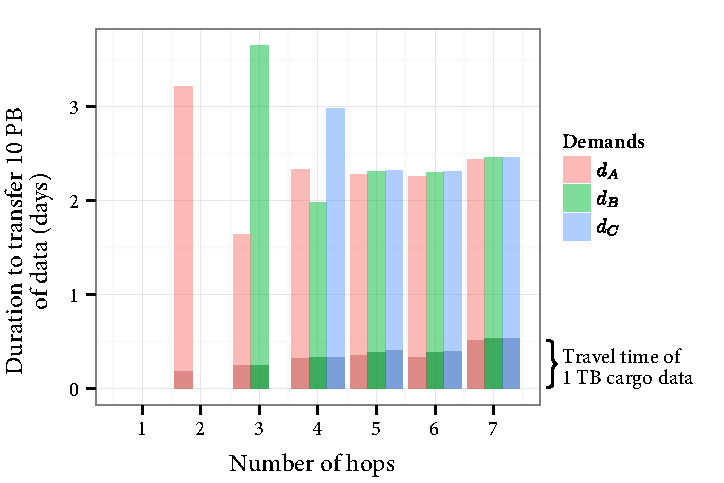
\includegraphics[width=8cm]{results/plot-france-3-transfers-duration.pdf}
    \caption{The duration needed to complete a 10~PB transfer (in lighter colors) and the travel time of a 1~TB data cargo (in darker colors) as a function of the candidate path maximal length in terms of hops.}
    \label{fig:hops-3-transfers-duration}
\end{wrapfigure}
We observe that none of the three destinations can be reached with a one-hop logical path. By increasing the logical path maximal length up to two hops, Lyon becomes the only city that can be reached, as shown in Figure~\ref{fig:france-demand-allocation}a. The high duration for $d_A$ is due to the low number of paths available and therefore of allocable vehicles, which results in a low throughput. If we consider logical paths of three hops or less, Bordeaux is now reachable in addition to Lyon. Figure~\ref{fig:france-demand-allocation}b shows that, in addition to the two-hop paths, there are more candidate paths between Paris and Lyon. As a result, more vehicles are allocated to $d_A$ which decreases its transfer duration. Regarding transfer $d_B$, the long transfer duration is explained by the few logical three-hop paths connecting Paris to Bordeaux in a similar way to $d_A$ and the logical paths of two-hop maximum length. With four-hop logical paths, Marseille is now also reachable, as shown in Figure~\ref{fig:france-demand-allocation}c. Nevertheless, the number of four-hop logical paths is still limited between Paris and Marseille, in a similar way as the two-hop paths to Lyon and the three-hop paths to Bordeaux. What is more, Marseille is located farther away from Paris compared to Lyon and $d_C$ competes for logical paths already passing by Lyon. This results in a longer transfer duration for $d_C$ but also in an increase of $d_A$ transfer duration.  At the same time, increasing the length of the candidate paths to four hops enables the allocation of more logical paths between Paris and Bordeaux, which results in a clear decrease in the transfer duration of $d_B$. This decrease is also explained by the low degree of similarity between the logical paths allocated to $d_B$ and those allocated to $d_A$ and $d_C$, as shown in Figure~\ref{fig:france-demand-allocation}c. Finally, with logical paths of five hops and more, the transfer durations are equivalent among all the demands. This further confirms that the strategy with controller guarantees a fair allocation in terms of throughput among all the demands. A slight increase in the transfer duration for all demands follows each increment in the number of hops as a direct consequence of the longer logical paths followed by all transfers. A similar trend can be observed for the travel time of the 1~TB cargo. 

\clearpage
\subsubsection{Cumulative capacity} 

We stress our system by allocating ten concurrent demands, all issued from Paris to the top nine other cities in France and one to Basel, Switzerland. This is shown in Figure~\ref{fig:10-demands-france}. We use the strategy with a controller to allocate the ten demands at the same time and consider again the \textsf{hop-by-hop} retransmission mechanism, given a 30\% data leakage for all logical links. We compute the cumulative throughput achieved by all ten transfers as a function of the length, expressed as the number of offloading spots of the logical paths allocated. We also compute the mean ratio of logical links shared by the logical paths allocated to each demand over the ones allocated to all other demands. The results are shown in Figure~\ref{fig:MMF-shared-throughput}. 

\begin{figure*}[!ht]
    \vspace{-15pt}
    \begin{subfigure}[b]{0.45\textwidth}
        \centering
        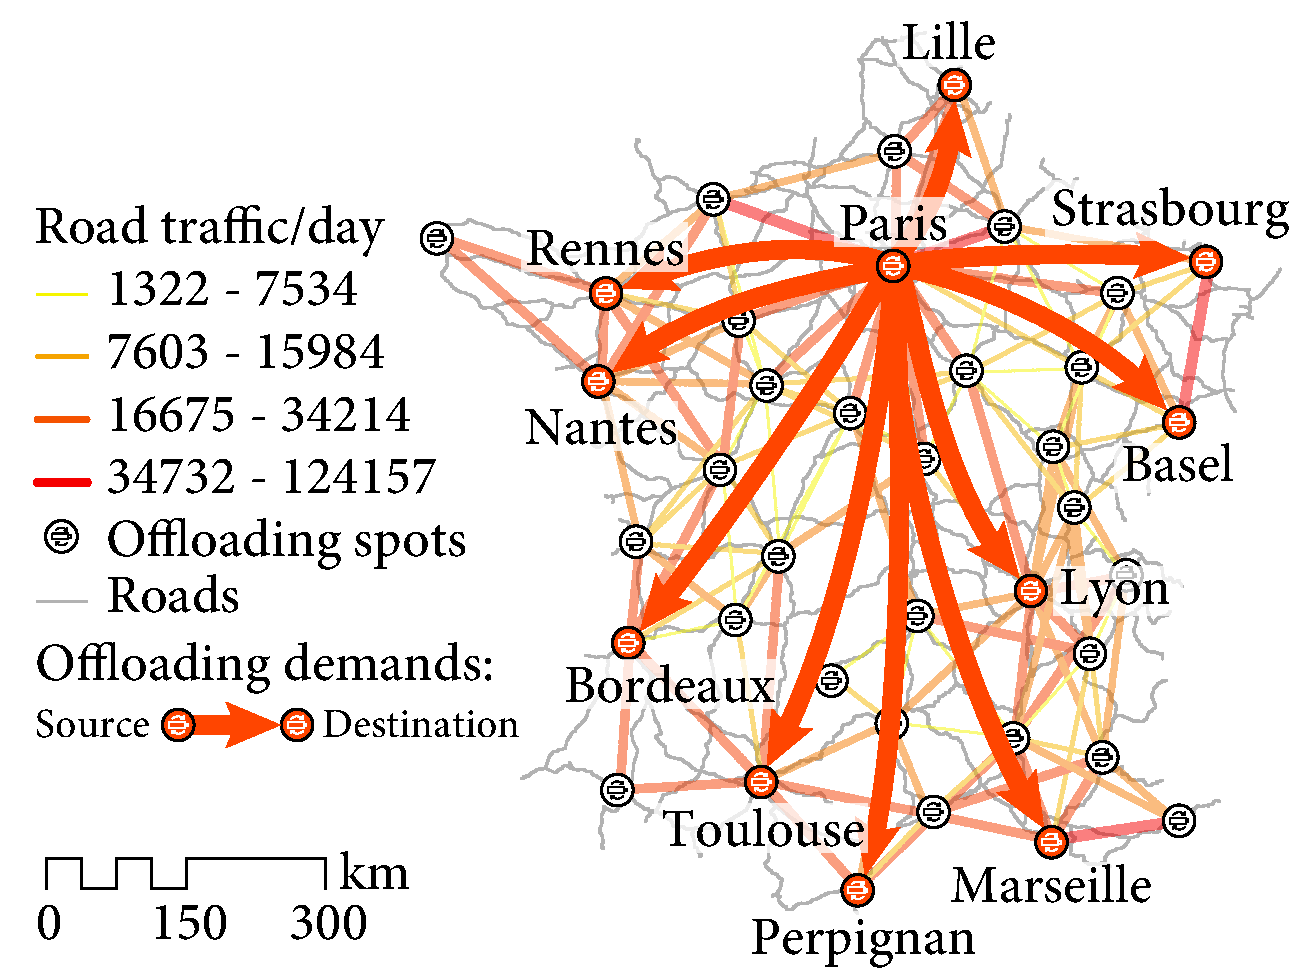
\includegraphics[width=\textwidth]{figures/France-overlay-transfers.pdf}
        \caption{Offloading demands to be allocated between Paris and the top ten other major cities of France, including Basel in Switzerland.}
        \label{fig:10-demands-france}
    \end{subfigure}%
    \qquad
    \begin{subfigure}[b]{0.45\textwidth}
        \centering
        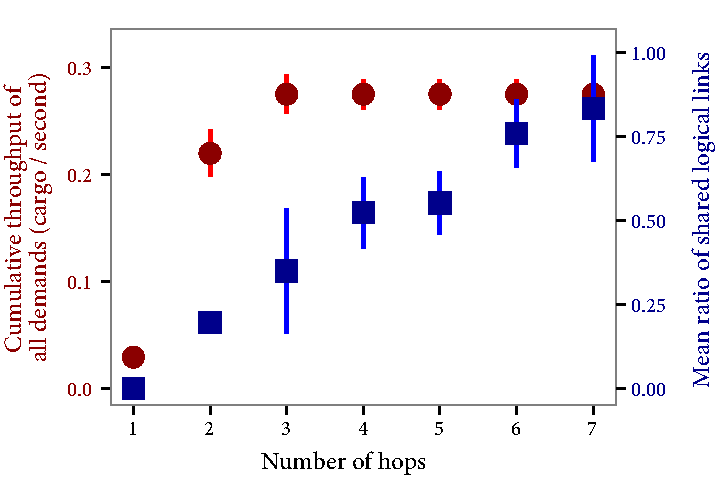
\includegraphics[width=\textwidth]{results/plot-france-MMF-shared-throughput.pdf}
        \caption{Cumulative throughput of the allocated demands and mean ratio of shared logical links between the allocated logical paths.}
        \label{fig:MMF-shared-throughput}
    \end{subfigure}%
    \caption{Cumulative capacity with ten offloading demands spanning the French road network.}
\end{figure*}

As for the previous case regarding demands $d_A$, $d_B$, and $d_C$, all ten destinations can be reached from Paris through logical paths of length at least three hops. With at least three-hop long logical links, the cumulative throughput of all ten demands reaches 280~Gbps and remains the same with a low standard deviation among all demands. The only city reachable by one-hop long logical paths is Lille while Lyon and Lille are the only cities reachable with paths of at two hops or less. As shown in Figure~\ref{fig:10-demands-france}, Lille is the closest to Paris compared to all other nine cities and can be reached by logical paths which exhibit the lowest degree of similarity with the paths connecting Paris to the other cities. For this reason, the transfer to Lille achieves a higher throughput compared to all other transfers. For the destinations located at least three hops away from Paris, the cumulative throughput remains the same even after increasing the number of hops of the allocable logical paths. Extending the length of the acceptable paths should allow the allocation of a higher number of paths to each demand and thus increase the cumulative throughput. However, most of the newly added paths are too long to be allocated or are already used for other transfers toward closer cities. For this reason, considering more paths by relaxing the length limit brings no benefit in terms of throughput. Considering longer paths to be allocable results in increased durations to complete the transfers. This further confirms the observation we made for Figure~\ref{fig:hops-3-transfers-duration}, \ie the strategy with controller allocates the paths to achieve fairness among all competing transfers.

\section{Discussions}
\label{sec:discuss-haulage}

\subsection{On the choice of traffic counts}
\label{sec:choice-traffic-counts}

\paragraph{\acrfull{aadt}.}
The purpose of our performance evaluation is to assess the capacity enhancement brought to the Internet by the road network. Our evaluation aims at determining the amount of data that can be transferred on the road within a given time period. A typical transfer lasts from a few days to a week, as we can offload up to one Petabyte. The traffic counts we use are provided by the \acrshort{aadt} (\textit{\acrfull{aadt}})\index{AADT}, which are yearly averages. As so, \acrshortpl{aadt} average out the effects of seasonal and diurnal variations or missing data due to flawed monitoring. To determine the traffic volume of a road segment over the duration of a transfer, we multiply the corresponding \acrshort{aadt} by the transfer duration measured in days. The use of the \acrshortpl{aadt} prevents our evaluation results from being affected by the diurnal, seasonal, or flawed bias. 

To transpose our work in a practical setting or commercial use, thinner-grained traffic count averages should be used to account for transfers lasting few hours or several weeks. An established practice for inferring traffic count averages for different time periods consists in using temporal allocation factors applied to the annual \acrshortpl{aadt}. 

An example of temporal allocation factors can be found in ``The Traffic Monitoring Guide'' where they are referred to as \textit{group factors}. These factors are provided by the US \acrfull{fhwa} to help State Department of Transportation plan their local \acrfull{hpms}~\cite{wright1997variability,guide2013us}. The guide describes how to calculate the factor groups (\ie temporal allocation factors) from the traffic data collected. The procedure depends on the location and the characteristics of the road segment, as well as the time period of interest. The traffic assignment models presented in this paper remain pertinent and can be used in combination with the temporal allocation factors.

The factors resulting from this procedure are applicable for time periods of several months (seasonal), days (day-of-week), or hours. These factors determine the road traffic pattern as a ratio of the \acrshort{aadt} for given road segments. The hourly vehicle volume $V_{i,\,t}$ on a road segment $i$ at time $t$ is estimated as the product of the average daily traffic $\textrm{AADT}_{i}$ and monthly $M_{g(i),\,t}$, daily $D_{g(i),\,t}$ and hourly $H_{g(i),\,t}$ factors, each for the factor group $g(i)$ of the road segment $i$:
\begin{equation}
    \label{eq:traffic-variation}
    V_{i,\,t} = \textrm{AADT}_{i} \times M_{g(i),\,t} \times D_{g(i),\,t} \times H_{g(i),\,t}.
\end{equation}
Note that the hourly factor takes into account the $D$-factor and the $K$-factor (directional and peak hour factors, respectively).

\paragraph{Finer-grain traffic counts.}
Another way to carry out the study of a dynamic system with finer-grain traffic counts (\eg in the order of the hour or for 15-minute intervals) is to characterize the dynamic flows of vehicles between offloading spots. Numerous works from transportation research have studied the estimation and prediction of dynamic origin-destination matrices using traffic counts, in particular, Bierlaire and Crittin or Casetta \etal both propose to do so using sequential estimator (namely Generalized Least Squares)~\cite{bierlaire2004efficient,cascetta1993dynamic}. With dynamic \acrshort{od} flows between the offloading spots, one can use the recent work~\cite{fleischer2007quickest} that built on Ford and Fulkerson~\cite{ford2015flows} to study the allocation of flows over time using time-expanded graphs. 

\section{Conclusion}
\label{sec:throughput-max-model-conclusions}

In this chapter, we presented a centralized architecture that implements the concept of vehicular offloading. This architecture consists of a controller in charge of configuring the road path consisting in the sequence of offloading spots involved in a data transfer. To determine this road path, the controller solves a vehicle flow allocation problem formulated with a max-min fairness model. This model guarantees fair allocation among competing demands and efficient utilization of the vehicular resources. To solve the vehicle flow allocation problem, the controller computes a logical representation of the road network. The output of the allocation problem is translated to a set of forwarding rules installed at the offloading spots. Those rules indicate how much data should be loaded on the vehicles depending on their direction of travel. The controller also implements mechanisms combining retransmissions and redundancy to ensure reliable data transfers. We evaluated the fairness of the allocation procedure as well as the throughput of the data transfers offloaded on the roads of France. To calculate the capacity of the roads we used elaborated traffic modelling techniques detailed in the Appendix~\ref{cha:traffic-forecasting-techniques} which provide more realistic values. 
We showed that an \acrshort{sdn} architecture provides the necessary elements to enable data offloading over the road network. With its holistic view of the offloading infrastructure, the architecture allows the management of a country-wide network, while keeping a fine-grained control of the data movements and its interactions with the vehicles to offload several Petabyte of data per day. Compared to the assessment study presented in Chapter~\ref{cha:feasibility-study}, the results we presented in this chapter benefit from the use of traffic modelling techniques combined with the use of a max-min fairness allocation model.
